\documentclass[twosided]{article}
\setlength{\oddsidemargin}{0.25 in}
\setlength{\evensidemargin}{-0.25 in}
\setlength{\topmargin}{-0.6 in}
\setlength{\textwidth}{6.5 in}
\setlength{\textheight}{8.5 in}
\setlength{\headsep}{0.75 in}
\setlength{\parindent}{0 in}
\setlength{\parskip}{0.1 in}

\usepackage{amsmath,amsfonts,graphicx,algorithm,caption}
\usepackage{cite}

\usepackage[document]{ragged2e}
\usepackage{graphicx}
\usepackage{subfigure}
\usepackage{mathtools}
\usepackage{algorithm,algorithmic}
\usepackage{amssymb,multirow,array,tikz}
\usepackage{epsfig,amsthm}
\usepackage{blkarray}
\usepackage{commath}
\usepackage[english]{babel}
\usepackage{url}

\newcounter{lecnum}
\renewcommand{\thepage}{\thelecnum-\arabic{page}}
\renewcommand{\thesection}{\thelecnum.\arabic{section}}
\renewcommand{\theequation}{\thelecnum.\arabic{equation}}
\renewcommand{\thefigure}{\thelecnum.\arabic{figure}}
\renewcommand{\thetable}{\thelecnum.\arabic{table}}
\makeatletter

\newcommand{\lecture}[4]{
   \pagestyle{myheadings}
   \thispagestyle{plain}
   \newpage
   \setcounter{lecnum}{#1}
   \setcounter{page}{1}
   \noindent
   \begin{center}
   \framebox{
      \vbox{\vspace{2mm}
    \hbox to 6.28in { {\bf IE643: Deep Learning : Theory and Practice
		\hfill Aug-Dec 2020} }
       \vspace{4mm}
       \hbox to 6.28in { {\Large \hfill Paper: #2  \hfill} }
       \vspace{2mm}
       \hbox to 6.28in { {\it Lecturer: #3 \hfill Scribes: #4} }
      \vspace{2mm}}
   }
   \end{center}
   \markboth{Lecture #1: #2}{Lecture #1: #2}

   {\bf Disclaimer}: {\it These notes have not been subjected to the
   usual scrutiny reserved for formal publications.  They may be distributed
   outside this class only with the permission of the Instructor.}
   \vspace*{4mm}
}

\begin{document}
\lecture{}{DeepVoice 2: Multi-Speaker Neural Text-to-Speech}{P. Balamurugan}{Shashank Kumar}

% \vspace{-0.7cm}
% \section*{Outline}
% \begin{itemize}
%     \item Motivation
%     \item Introduction
%     \item Methodologies
%     \item Experiments
%     \item Results
%     \item References
% \end{itemize}

\section*{Motivation}
Text-to-speech (TTS) synthesis has a variety of applications ranging from communication devices, digitally talking bots to media broadcasting like smart TVs and even to IoT. The technology is expanding to other industries like finance, health care, e-learning, telecommunication and robotics. Most TTS systems are built for a single artificial voice and multi-speaker voice systems require much more data and efforts.  

\section*{Introduction}
The paper proposes to an all-neural multi-speaker TTS system. The model aims to solve the multi-speaker TTS problem by using a single model, and a lot less data per speaker when compared to single-speaker systems. The paper is based on the following two elements - \\
    \begin{enumerate}
        \item \textbf{DeepVoice 2 \cite{DeepVoice2}}, an architecture improved upon \textbf{DeepVoice 1\cite{DeepVoice1}}
        \item A \textbf{WaveNet-based \cite{WaveNet}} spectrogram-to-audio neural vocoder which is used with \textbf{Tacotron \cite{Tacotron}}
    \end{enumerate}
The general structure is the same as DeepVoice 1. The neural network creates trainable speaker embeddings  into DeepVoice2 and Tacotron using the single speaker models as a  baseline. The network to capture speaker embeddings for the speaker characteristics is trained from scratch.

\section*{Methodologies}
The text is first converted into phonemes using pronunciation dictionary, which are then fed for duration prediction, upscaling and generating the frequency $F0$. This frequency is finally passed to the vocal model for speech synthesis. 
    \begin{figure}[h]
        \centering
        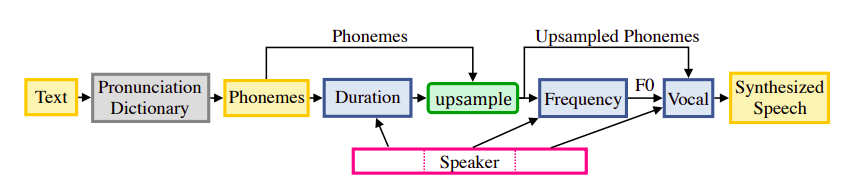
\includegraphics[width=0.7\textwidth]{images/Figure1.png}
        \caption{Inference system diagram}
        \label{fig:figure1}
    \end{figure}

For the multi speaker task, each of the models is augmented with a single low-dimensional speaker embedding vector per speaker, thus allowing near-complete weight sharing between speakers. Each model has its own set of speaker embeddings, which are incorporated into multiple portions of the model. The following sections describe the models proposed by the paper for the TTS task.

\subsection*{Segmentation Model}
Estimation of phoneme locations is formulated as an unsupervised learning task. The segmentation model uses a \textbf{convolutional-recurrent architecture} with \textbf{connectionist-temporal-classification (CTC) loss \cite{CTCLoss}}. The phoneme pairs are first classified and then the boundary is extracted between them. The major change in DeepVoice 2 as compared to DeepVoice 1 is the use of batch-normalization and residual connections in the convolutional layers.
    \begin{align*}
	    h^{(l)} = relu(h^{(l)} + BN(W^{(l)} * h^{(l-1)}))
	\end{align*}
where $h^{(l)}$ is the output of the $l$-th layer, $W^{(l)}$ is the convolutional filterbank, $*$ is the convolutional operation and $BN$ is the \textbf{batch-normalization operation \cite{BatchNorm}}.\\
For the multi-speaker task, batch-normalized activations are multiplied by site-specific speaker embedding $g_s$, which is shared by all the layers.
    \begin{align*}
	    h^{(l)} = relu(h^{(l)} + BN(W^{(l)} * h^{(l-1)}) \cdot g_s)
	\end{align*}

\subsection*{Duration Model}
Duration prediction is modelled as a sequence labeling problem using \textbf{conditional random field (CRF) \cite{CRF}}. The phonemes are assigned into log-scaled buckets. Quantizing the duration prediction and introducing pairwise dependence implied by CRF improves synthesis quality. \\ 
The multi-speaker model uses speaker-dependent t recurrent initialization and input augmentation. A site-specific embedding is used to initialize RNN hidden states, and another site-specific embedding is provided as input to the first RNN layer by concatenating it to the feature vectors.

\subsection*{Frequency Model}
The predicted phoneme durations are upsampled from a per-phoneme input features to a per-frame input for the frequency model. Each frame is of 10ms. Phonemes are either extended or split into multiple frames so as to maintain the size of 10ms. DeepVoice 2 consists of two layers. Firstly, $f_{GRU}$ is predicted by a single layer bidirectional \textbf{gated recurrent unit (GRU) \cite{GRU}} followed by affine projection. The second prediction, $f_{CONV}$ is made by adding up the contributions of multiple convolutions with varying convolution widths and a single output channel.
    \begin{align*}
	    f = \omega \cdot f_{GRU} + (1 - \omega) \cdot f_{CONV}
	\end{align*}
where $\omega$ is the mixture ratio predicted from the hidden state using an affine projection and a sigmoid activation.
The normalized prediction $f$ is converted is converted to true frequency $F_0$ prediction as follows.
    \begin{align*}
	    F_0 = \mu_{F_0} + \sigma_{F_0} \cdot f
	\end{align*}
where $\mu_{F_0}$ and $\sigma_{F_0}$ are the mean and standard deviation of $F_0$, respectively.\\
The multi-speaker model uses recurrent intialization with a single site-specific speaker-embedding. The mean ($\mu_{F0}$) and standard deviation ($\sigma_{F_0}$) are made as trainable parameters.
    \begin{align*}
	    F_0 = \mu_{F_0} \cdot (1 + softsign(V_{\mu}^Tg_f)) + \sigma_{F_0} \cdot (1 + softsign(V_{\sigma}^Tg_f)) \cdot f
	\end{align*}
where $g_f$ is a site-specific speaker embedding, $\mu_{F_0}$ and $\sigma_{F_0}$ are trainable scalar parameters initialized
to the $F_0$ mean and standard deviation on the dataset, and $V_{\mu}$ and $V_{\sigma}$ are trainable parameter vectors.

\subsection*{Vocal Model}
The vocal model is based on \textbf{WaveNet architecture} with a two-layer bidirectional \textbf{QRNN \cite{QRNN}} conditioning network. The  1 x 1 convolution between the gated tanh nonlinearity and the residual connection is removed and the same conditioner bias for every layer of the WaveNet is used, instead of generating a separate bias for every layer as was done in Deep Voice 1.\\
The multi-speaker vocal model uses only input augmentation, with the site-specific speaker embedding concatenated onto each input frame of the conditioner

\begin{figure}[h]
    \centering
    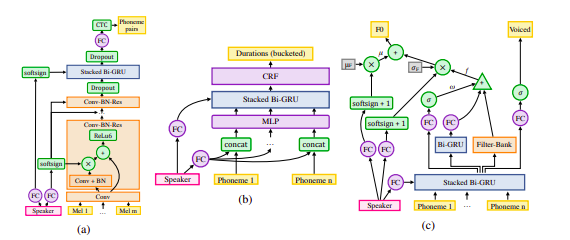
\includegraphics[width=\textwidth]{images/Figure2.png}
    \caption{Multi-speaker architecture for (a)segmentation,  (b) duration (c) frequency models}
    \label{fig:figure2}
\end{figure}

\section*{Experiments}
\begin{itemize}
    \item All the aforementioned models are trained on the \textbf{VCTK dataset} with 44 hours of speech, which contains 108 speakers with approximately 400 utterances each. The models are also trained on an internal dataset of audiobooks, which contains 477 speakers with 30 minutes of audio each (for a total of 238 hours).
    \item To incorporate each speaker’s unique voice signature to influence the model, the speaker embeddings are injected into multiple portions of the model. The following patterns tend to improve the performance.
    \begin{itemize}
        \item \textbf{Site-Specific Speaker Embeddings:} For every use site in the model architecture, transform the shared speaker embedding to the appropriate dimension and form through an affine projection and a non-linearity.
        \item \textbf{Recurrent Initialization:} Initialize recurrent layer hidden states with site-specific speaker embeddings.
        \item \textbf{Input Augmentation:} Concatenate a site-specific speaker embedding to the input at every timestep of a recurrent layer.
        \item \textbf{Feature Gating:} Multiply layer activations element-wise with a site-specific speaker embedding to render adaptable information flow.
    \end{itemize}
    \item In the \textbf{segmentation model}, the same site-specific embedding is shared for all the convolutional layers. In addition, the recurrent layers are initialized with a second site specific embedding. Each layer shares the same site-specific embedding, rather than having a separate embedding per layer.
    \item The \textbf{vocal model} is able to generate somewhat distinct-sounding voices even without speaker embeddings because of the distinctive features provided by the frequency and duration models. But having speaker embeddings in the vocal model increases the audio quality significantly.
    \item When training \textbf{multi-speaker Tacotron} variants, the model performance is highly dependent on model hyperparameters, and that some models often fail to learn attention mechanisms for a small subset of speakers. Due to the sensitivity of the model to hyperparameters and data.
    \item If the speech in each audio clip does not start at the same timestep, the models are much less likely to converge to a meaningful attention curve and recognizable speech. Thus, all initial and final silence is trimmed in each audio clip
    \item The \textbf{Tacotron character-to-spectrogram architecture} consists of a convolution-bank-highway-GRU (CBHG) encoder, an attentional decoder, and a CBHG post-processing network. Incorporating speaker embeddings into the CBHG post-processing network degrades output quality, whereas incorporating speaker embeddings into the character encoder is necessary. Augmenting the attentional decoder with speaker embeddings is helpful. 
    \item A \textbf{Wavenet-based neural vocoder} produces higher quality audio from linear spectrograms than the original \textbf{Griffin-Lim algorithm} used in Tacotron. The architecture for the same is as shown below.
\end{itemize}

\section*{Results}
\subsection*{Single-speaker speech synthesis}
To compare the results, MOS evaluations using the \textbf{CrowdMOS framework \cite{CrowdMOS}} is used. The results show conclusively that the DeepVoice 2 architecture improves the quality significantly over DeepVoice 1. The table also demonstrate that converting Tacotron-generated spectrograms to audio using WaveNet is preferable to using the iterative Griffin-Lim algorithm. The results are summarized in the table below with 95\% confidence intervals. 
    \begin{center}
        \begin{tabular}{||c c c||} 
        \hline
        \textbf{Model} & \textbf{Sample Frequency} & \textbf{MOS} \\ [0.7ex] 
        \hline\hline
        DeepVoice 1 & 16KHz & 2.05 \pm 0.24 \\ 
        \hline
        DeepVoice 2 & 16KHz & 2.96 \pm 0.38 \\
        \hline
        Tacotron (Griffin-Lim) & 24KHz & 2.57 \pm 0.28 \\
        \hline
        Tacotron (WaveNet) & 24KHz & 4.17 \pm 0.18 \\
        \hline
        \end{tabular}
    \end{center}

\subsection*{Multi-speaker speech synthesis}
MOS evaluations are used as in the single-speaker case in order to evaluate the quality of the synthesized audio, 
framework, and the results are summarized below. The Deep Voice 2 model can approach an MOS value that is close to the ground truth, when low sampling rate and companding/expanding taken into account.
    \begin{center}
        \begin{tabular}{||c c c c c||} 
        \hline
        \textbf{Dataset} & \textbf{Multi-Speaker Model} & \textbf{Sample Frequency} & \textbf{MOS} & \textbf{Accuracy} \\ [0.7ex] 
        \hline\hline
        VCTK & DeepVoice 2 (20-layer WaveNet) & 16KHz & 2.8 \pm 0.13 & 99.9\% \\
        \hline
        VCTK & DeepVoice 2 (40-layer WaveNet) & 16KHz & 3.21 \pm 0.13 & 100\% \\
        \hline
        VCTK & DeepVoice 2 (60-layer WaveNet) & 16KHz & 3.42 \pm 0.12 & 99.7\% \\
        \hline
        VCTK & DeepVoice 2 (80-layer WaveNet) & 16KHz & 3.53 \pm 0.12 & 99.9\% \\
        \hline
        VCTK & Tacotron (Griffin-Lim) & 24KHz & 1.68 \pm 0.12 & 99.4\% \\
        \hline
        VCTK & Tacotron (20-layer WaveNet) & 24KHz & 2.51 \pm 0.13 & 60.9\% \\
        \hline
        VCTK & Ground Truth Data & 48KHz & 4.65 \pm 0.06 & 99.7\% \\
        \hline
        Audiobooks & Deep Voice 2 (80-layer WaveNet) & 16KHz & 2.97 \pm 0.17 & 97.4\% \\
        \hline
        Audiobooks & Tacotron (Griffin-Lim) & 24KHz & 1.73 \pm 0.22 & 93.9\% \\
        \hline
        Audiobooks & Tacotron (20-layer WaveNet) & 24KHz & 2.11 \pm 0.20 & 66.5\% \\
        \hline
        Audiobooks & Ground Truth Data & 44.1KHz & 4.63 \pm 0.04 & 98.8\% \\
        \hline
        \end{tabular}
    \end{center}

\begin{figure}[h]
    \centering
    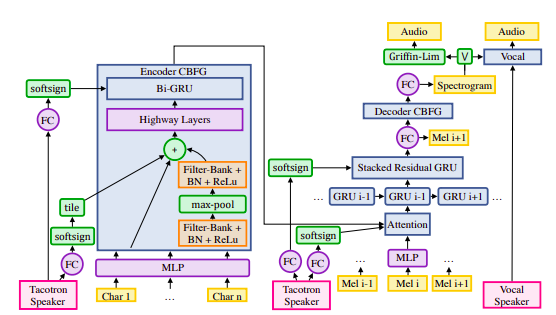
\includegraphics[width=0.8\textwidth]{images/Figure3.png}
    \caption{Tacotron with speaker conditioning in the encoder CBHG module and decoder with two wats to convert spectrogram to audio: Griffin-Lim or our speaker-conditioned vocal model}
    \label{fig:figure2}
\end{figure}

\section*{Conclusions}
The paper explores on how entirely-neural speech synthesis pipelines may be extended to multispeaker TTS via low-dimensional trainable speaker embeddings. It presents DeepVoice 2, an improved single-speaker model. Next, it demonstrates the applicability of the technique by training both multi-speaker Deep Voice 2 and multi-speaker Tacotron models, and evaluate their quality through MOS. In conclusion, the speaker embedding technique can be used to create high quality TTS systems and conclusively show that neural speech synthesis models can learn effectively from small amounts of data spread among hundreds of different speakers.

\subsection*{How the paper helped with the project?}
The predecessor of the paper - \textbf{DeepVoice 1: Real-time neural Text-To-Speech} marked the beginning of the journey of speech synthesis based on neural networks. \textbf{DeepVoice 2: Multi-Speaker Neural Text-to-Speech} took it a step further by expanding the horizon to multiple speakers. \textbf{DeepVoice 3: Scaling Text-to-Speech with Convolutional Sequence Learning \cite{DeepVoice3}} took it even a step further. The project paper assigned to us is \textbf{Transfer Learning from Speaker Verification to Multispeaker Text-To-Speech Synthesis \cite{TransferLearning}}. This paper draws inspiration from the results achieved in DeepVoice series of papers, specifically DeepVoice 2 and DeepVoice 3. DeepVoice 2 helper us understand the foundations laid by it in the field of multi-speaker TTS. 
    
\begin{thebibliography}{99}
\bibitem{DeepVoice2}
\textit{Deep Voice 2: Multi-Speaker Neural Text-to-Speech, 2017}
Sercan Arik and Gregory Diamos and Andrew Gibiansky and John Miller and Kainan Peng and Wei Ping and Jonathan Raiman and Yanqi Zhou
\bibitem{DeepVoice3}
\textit{Deep Voice 3: Scaling Text-to-Speech with Convolutional Sequence Learning, 2018}
Wei Ping, Kainan Peng, Andrew Gibiansky, Sercan O. Arik, Ajay Kannan, Sharan Narang, Jonathan Raiman, John Miller
\bibitem{DeepVoice1}
\textit{Deep voice: Real-time neural text-to-speech, 2017}
S. O. Arik, M. Chrzanowski, A. Coates, G. Diamos, A. Gibiansky, Y. Kang, X. Li, J. Miller, J. Raiman, S. Sengupta, and M. Shoeybi
\bibitem{TransferLearning}
\textit{Transfer Learning from Speaker Verification to Multispeaker Text-To-Speech Synthesis, 2019}
Ye Jia, Yu Zhang, Ron J. Weiss, Quan Wang, Jonathan Shen, Fei Ren, Zhifeng Chen, Patrick Nguyen, Ruoming Pang, Ignacio Lopez Moreno, Yonghui Wu
\bibitem{WaveNet}
\textit{Wavenet: A generative model for raw audio, 2016}
A. v. d. Oord, S. Dieleman, H. Zen, K. Simonyan, O. Vinyals, A. Graves, N. Kalchbrenner, A. Senior, and K. Kavukcuoglu
\bibitem{Tacotron}
\textit{Tacotron: Towards end-to-end speech synthesis, 2017}
Y. Wang, R. Skerry-Ryan, D. Stanton, Y. Wu, R. J. Weiss, N. Jaitly, Z. Yang, Y. Xiao, Z. Chen, S. Bengio
\bibitem{CTCLoss}
\textit{Connectionist temporal classification: labelling unsegmented sequence data with recurrent neural networks, 2006}
A. Graves, S. Fernández, F. Gomez, and J. Schmidhuber
\bibitem{BatchNorm}
\textit{Batch normalization: Accelerating deep network training by reducing internal covariate shift, 2015}
S. Ioffe and C. Szegedy
\bibitem{CRF}
\textit{Neural architectures for named entity recognition, 2016}
G. Lample, M. Ballesteros, K. Kawakami, S. Subramanian, and C. Dyer
\bibitem{GRU}
\textit{Learning phrase representations using rnn encoder-decoder for statistical machine translation}
K. Cho, B. Van Merriënboer, C. Gulcehre, D. Bahdanau, F. Bougares, H. Schwenk, and Y. Bengio
\bibitem{QRNN}
\textit{Quasi-recurrent neural networks, 2017}
J. Bradbury, S. Merity, C. Xiong, and R. Socher
\bibitem{CrowdMOS}
\textit{Crowdmos: An approach for crowdsourcing mean opinion score studies, 2011}
F. Ribeiro, D. Florêncio, C. Zhang, and M. Seltzer
\end{thebibliography}

\end{document}
